\subsection{Tutorial 2: Pulling on a carbon nanotube}
\label{carbon-nanotube-label}

\begin{figure}
{\centering
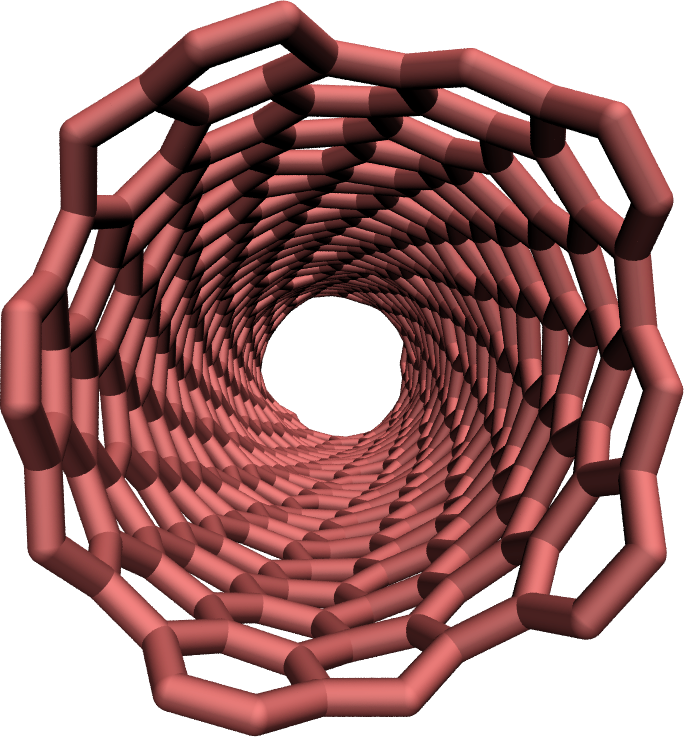
\includegraphics[width=0.55\linewidth]{CNT}
\caption{Snapshot of the carbon nanotube (CNT) made using VMD.}}
\label{fig:CNT}
\end{figure}

\vspace{0.25cm} \noindent The objective of this tutorial is to impose the deformation of a carbon nanotube (CNT) using LAMMPS. In this tutorial, a small carbon nanotube (CNT) is simulated within an empty box using LAMMPS (Fig.\,\ref{fig:CNT}). An external forcing is imposed on the CNT, and its deformation is measured with time. The difference between classical and reactive force fields
is illustrated through this tutorial. With a classical force field, the bonds between atoms are unbreakable. With the reactive force field (named AIREBO \cite{stuart2000reactive}), the breaking of the chemical bonds is possible when the imposed deformation is strong enough.

\subsubsection{Unbreakable bonds}
\noindent With most classical molecular dynamics force fields, the chemical bonds between the atoms are set at the start of the simulation. Regardless of the forces applied to the atoms during the simulations, the bonds remain intact. The bonds between neighbor atoms typically consist of springs with given equilibrium distances $r_0$ and a constant $k_b$: $U_b = k_b \left( r - r_0 \right)^2$.
Additionally, angular and dihedral constraints are usually applied to maintain the relative orientations of neighbor atoms. 

Download directly the CNT topology by clicking \href{https://lammpstutorials.github.io/lammpstutorials-inputs/level1/breaking-a-carbon-nanotube/unbreakable-bonds/cnt_molecular.data}{here}. It was created using VMD and TopoTools \cite{kohlmeyer2017topotools}, and contains information about the positions of the carbon atoms, as well as the
identity of the atoms that are linked by \textit{bonds}, \textit{angles}, \textit{dihedrals},
and \textit{impropers} constraints. Save the \textit{cnt$\_$molecular.data} file
in a folder named \textit{unbreakable-bonds/}.

\paragraph{The LAMMPS input}
Create a new text file within \textit{unbreakable-bonds/} and name it \textit{input.lammps}. Copy the following lines in it:
\begin{verbatim}
variable T equal 300

units real
atom_style molecular
boundary f f f
pair_style lj/cut 14

bond_style harmonic
angle_style harmonic
dihedral_style opls
improper_style harmonic

special_bonds lj 0.0 0.0 0.5

read_data cnt_molecular.data
\end{verbatim}
The chosen unit system is \textit{real} (therefore distances are in Ångstrom, time in femtosecond), the \textit{atom$\_$style} is molecular (therefore atoms are dots that can be bonded with each other), and the boundary conditions are fixed. The boundary conditions do not matter here, as the box boundaries were placed far from the CNT. 

Just like in the previous tutorial, \hyperref[lennard-jones-label]{Lennard Jones fluid}, the pair style is \textit{lj/cut} (i.e. a Lennard-Jones potential with a short-range cutoff) with parameter 14, which means that only the atoms closer than 14 Ångstroms from each other interact through a Lennard-Jones potential. The \textit{bond$\_$style}, \textit{angle$\_$style}, \textit{dihedral$\_$style}, and \textit{improper$\_$style} commands specify the different potentials used to restrain the relative positions of the atoms. For more details about the potentials used here, you can have a look at the LAMMPS website. The \textit{special$\_$bonds} command sets the weighting factors for the Lennard-Jones interaction between atoms directly connected by a bond, separated by two bonds, and separated by three bonds, respectively. The last command, \textit{read$\_$data}, imports the \textit{cnt$\_$molecular.data} file previously generated with VMD, which contains the information about the box size, atom positions, etc.